\XtoCBlock{Sin3Gen}
\label{block:Sin3Gen}
\begin{figure}[H]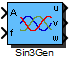
\includegraphics{Sin3Gen}\end{figure} 

\begin{XtoCtabular}{Inports}
A & Amplitude\tabularnewline
\hline
f & Frequency\tabularnewline
\hline
\end{XtoCtabular}


\begin{XtoCtabular}{Outports}
u & Sine wave output phase u\tabularnewline
\hline
v & Sine wave output phase v\tabularnewline
\hline
w & Sine wave output phase w\tabularnewline
\hline
\end{XtoCtabular}

\begin{XtoCtabular}{Mask Parameters}
fmax & Maximum Frequency in Hz\tabularnewline
\hline
Offset & Offset\tabularnewline
\hline
ts\_fact & Multiplication factor of base sampling time (in integer format)\tabularnewline
\hline
\end{XtoCtabular}

\subsubsection*{Description:}
Generation of a 3 sine waves with amplitude (A) and frequency (f).

% include optional documentation file
\InputIfFileExists{\XcHomePath/Library/General/Doc/Sin3Gen_Info.tex}{\vspace{1ex}}{}

\subsubsection*{Implementations:}
\begin{tabular}{l l}
\textbf{FiP8} & 8 Bit Fixed Point Implementation\tabularnewline
\textbf{FiP16} & 16 Bit Fixed Point Implementation\tabularnewline
\textbf{FiP32} & 32 Bit Fixed Point Implementation\tabularnewline
\textbf{Float32} & 32 Bit Floating Point Implementation\tabularnewline
\textbf{Float64} & 64 Bit Floating Point Implementation\tabularnewline
\end{tabular}

\XtoCImplementation{FiP8}
\index{Block ID!432}
\nopagebreak[0]
% Implementation details
\begin{tabular}{l l}
\textbf{Name} & FiP8 \tabularnewline
\textbf{ID} & 432 \tabularnewline
\textbf{Revision} & 1.0 \tabularnewline
\textbf{C filename} & Sin3Gen\_FiP8.c \tabularnewline
\textbf{H filename} & Sin3Gen\_FiP8.h \tabularnewline
\end{tabular}
\vspace{1ex}

8 Bit Fixed Point Implementation

\begin{XtoCtabular}{Controller Parameters}
delta\_phi & Angle increment\tabularnewline
\hline
offset & Amplitude offset\tabularnewline
\hline
phi & Current angle\tabularnewline
\hline
\end{XtoCtabular}

% Implementation data structure
\XtoCDataStruct{Data Structure:}
\begin{lstlisting}
typedef struct {
     uint16        ID;
     int8          *A;
     int8          *f;
     int8          u;
     int8          v;
     int8          w;
     int8          delta_phi;
     int8          offset;
     int8          phi;
} SIN3GEN_FIP8;
\end{lstlisting}

\ifdefined \AddTestReports
\InputIfFileExists{\XcHomePath/Library/General/Doc/Test_Sin3Gen_FiP8.tex}{}{}
\fi
\XtoCImplementation{FiP16}
\index{Block ID!433}
\nopagebreak[0]
% Implementation details
\begin{tabular}{l l}
\textbf{Name} & FiP16 \tabularnewline
\textbf{ID} & 433 \tabularnewline
\textbf{Revision} & 1.0 \tabularnewline
\textbf{C filename} & Sin3Gen\_FiP16.c \tabularnewline
\textbf{H filename} & Sin3Gen\_FiP16.h \tabularnewline
\end{tabular}
\vspace{1ex}

16 Bit Fixed Point Implementation

\begin{XtoCtabular}{Controller Parameters}
delta\_phi & Angle increment\tabularnewline
\hline
offset & Amplitude offset\tabularnewline
\hline
phi & Current angle\tabularnewline
\hline
\end{XtoCtabular}

% Implementation data structure
\XtoCDataStruct{Data Structure:}
\begin{lstlisting}
typedef struct {
     uint16        ID;
     int16         *A;
     int16         *f;
     int16         u;
     int16         v;
     int16         w;
     int16         delta_phi;
     int16         offset;
     int16         phi;
} SIN3GEN_FIP16;
\end{lstlisting}

\ifdefined \AddTestReports
\InputIfFileExists{\XcHomePath/Library/General/Doc/Test_Sin3Gen_FiP16.tex}{}{}
\fi
\XtoCImplementation{FiP32}
\index{Block ID!434}
\nopagebreak[0]
% Implementation details
\begin{tabular}{l l}
\textbf{Name} & FiP32 \tabularnewline
\textbf{ID} & 434 \tabularnewline
\textbf{Revision} & 1.0 \tabularnewline
\textbf{C filename} & Sin3Gen\_FiP32.c \tabularnewline
\textbf{H filename} & Sin3Gen\_FiP32.h \tabularnewline
\end{tabular}
\vspace{1ex}

32 Bit Fixed Point Implementation

\begin{XtoCtabular}{Controller Parameters}
delta\_phi & Angle increment\tabularnewline
\hline
offset & Amplitude offset\tabularnewline
\hline
phi & Current angle\tabularnewline
\hline
\end{XtoCtabular}

% Implementation data structure
\XtoCDataStruct{Data Structure:}
\begin{lstlisting}
typedef struct {
     uint16        ID;
     int32         *A;
     int32         *f;
     int32         u;
     int32         v;
     int32         w;
     int32         delta_phi;
     int32         offset;
     int32         phi;
} SIN3GEN_FIP32;
\end{lstlisting}

\ifdefined \AddTestReports
\InputIfFileExists{\XcHomePath/Library/General/Doc/Test_Sin3Gen_FiP32.tex}{}{}
\fi
\XtoCImplementation{Float32}
\index{Block ID!435}
\nopagebreak[0]
% Implementation details
\begin{tabular}{l l}
\textbf{Name} & Float32 \tabularnewline
\textbf{ID} & 435 \tabularnewline
\textbf{Revision} & 0.1 \tabularnewline
\textbf{C filename} & Sin3Gen\_Float32.c \tabularnewline
\textbf{H filename} & Sin3Gen\_Float32.h \tabularnewline
\end{tabular}
\vspace{1ex}

32 Bit Floating Point Implementation

\begin{XtoCtabular}{Controller Parameters}
delta\_phi & Angle increment\tabularnewline
\hline
offset & Amplitude offset\tabularnewline
\hline
phi & Current angle\tabularnewline
\hline
\end{XtoCtabular}

% Implementation data structure
\XtoCDataStruct{Data Structure:}
\begin{lstlisting}
typedef struct {
     uint16        ID;
     float32       *A;
     float32       *f;
     float32       u;
     float32       v;
     float32       w;
     float32       delta_phi;
     float32       offset;
     float32       phi;
} SIN3GEN_FLOAT32;
\end{lstlisting}

\ifdefined \AddTestReports
\InputIfFileExists{\XcHomePath/Library/General/Doc/Test_Sin3Gen_Float32.tex}{}{}
\fi
\XtoCImplementation{Float64}
\index{Block ID!436}
\nopagebreak[0]
% Implementation details
\begin{tabular}{l l}
\textbf{Name} & Float64 \tabularnewline
\textbf{ID} & 436 \tabularnewline
\textbf{Revision} & 0.1 \tabularnewline
\textbf{C filename} & Sin3Gen\_Float64.c \tabularnewline
\textbf{H filename} & Sin3Gen\_Float64.h \tabularnewline
\end{tabular}
\vspace{1ex}

64 Bit Floating Point Implementation

\begin{XtoCtabular}{Controller Parameters}
delta\_phi & Angle increment\tabularnewline
\hline
offset & Amplitude offset\tabularnewline
\hline
phi & Current angle\tabularnewline
\hline
\end{XtoCtabular}

% Implementation data structure
\XtoCDataStruct{Data Structure:}
\begin{lstlisting}
typedef struct {
     uint16        ID;
     float64       *A;
     float64       *f;
     float64       u;
     float64       v;
     float64       w;
     float64       delta_phi;
     float64       offset;
     float64       phi;
} SIN3GEN_FLOAT64;
\end{lstlisting}

\ifdefined \AddTestReports
\InputIfFileExists{\XcHomePath/Library/General/Doc/Test_Sin3Gen_Float64.tex}{}{}
\fi
